\documentclass[10pt]{article}
\usepackage[margin=2.4cm]{geometry}
\usepackage{graphicx,booktabs,amsmath,amssymb,microtype}
\usepackage[hidelinks]{hyperref}
\usepackage{xcolor}
\setlength{\parskip}{4pt}\setlength{\parindent}{0pt}
\title{\textbf{Unit-Nets Day 2:\\A Language Model You Can Read With
Arithmetic}}
\author{Remy \& Claude}
\date{July 8, 2026 \quad \texttt{\small~/Code/unit-net}
 \ \texttt{\small~/Code/j-carve}}
\begin{document}\maketitle

\section{Context}
Sequel to \emph{One Day of Training Without Gradients} (the constrained
``unit-net'' geometry: convex excitatory rows, bounded inhibition, dual
projections, activations in $[0,1]$). Anthropic's J-lens (July 2026) reads
what an internal state is disposed to say via a corpus-averaged Jacobian,
$\mathrm{lens}_l(h) = \mathrm{unembed}(J_l h)$,
$J_l = \mathbb{E}[\partial h_{\mathrm{final}}/\partial h_l]$ --- averaged
because a transformer's layer-to-output map is input-dependent. Remy's
hypothesis: in a unit-net the true Jacobian is \textbf{exact per input and
bounded in fixed units} --- the workspace is readable off the wiring, no
fitting required. Today: distill Qwen2.5-0.5B into a unit-net and run the
J-space program on it.

\section{The student}
\texttt{TokenUnitLM}: a shared token table (each feature unit a convex
attention budget over the vocabulary) feeding a unit-net trunk; 12-token
context, reduced 2{,}048-token vocabulary (96.4\% corpus coverage),
distilled on TinyStories by KL + hard-target CE. A flat one-hot design
fails structurally (13 hot inputs among 24{,}577 --- convex rows never see
the tokens); the table architecture fixes it.

\section{The distillation gauntlet}
\begin{center}\small\begin{tabular}{@{}p{4.2cm}p{2.6cm}p{7.4cm}@{}}\toprule
Run & Result & Lesson\\\midrule
Mirror descent, hot schedule & oscillates $0.5\%\!\leftrightarrow\!33\%$ &
multiplicative simplex updates need short, cooled schedules\\
Both trainers, ``33\%'' & \textbf{artifact} & the UNK slot had been given
the logsumexp of 149k excluded tokens --- teacher argmax \emph{was} UNK
$\sim$1/3 of the time; both students learned to say UNK forever\\
Clean targets, ReLU & 6--10\%, rank-28 affine & optimizer kills 484/512
units via inhibition overgrowth (the \emph{lazy-linear minimum})\\
Sigmoid rescue & 17.1\% & sigmoid cannot die and auto-normalizes scale;
lens becomes local-only (\S4)\\
\textbf{Hardened ReLU} & \textbf{32.9\%} & concentrated init + inhibition
row-sum cap + liveness auxiliary: dead $=0$ for 14k steps \emph{and}
exact decomposition restored\\
\bottomrule\end{tabular}\end{center}

Final student: 33.2\% teacher agreement@1, 25.5\% next-token accuracy ---
a functional TinyStories LM in fully constrained, verifier-legal weights.

\begin{figure}[h]\centering
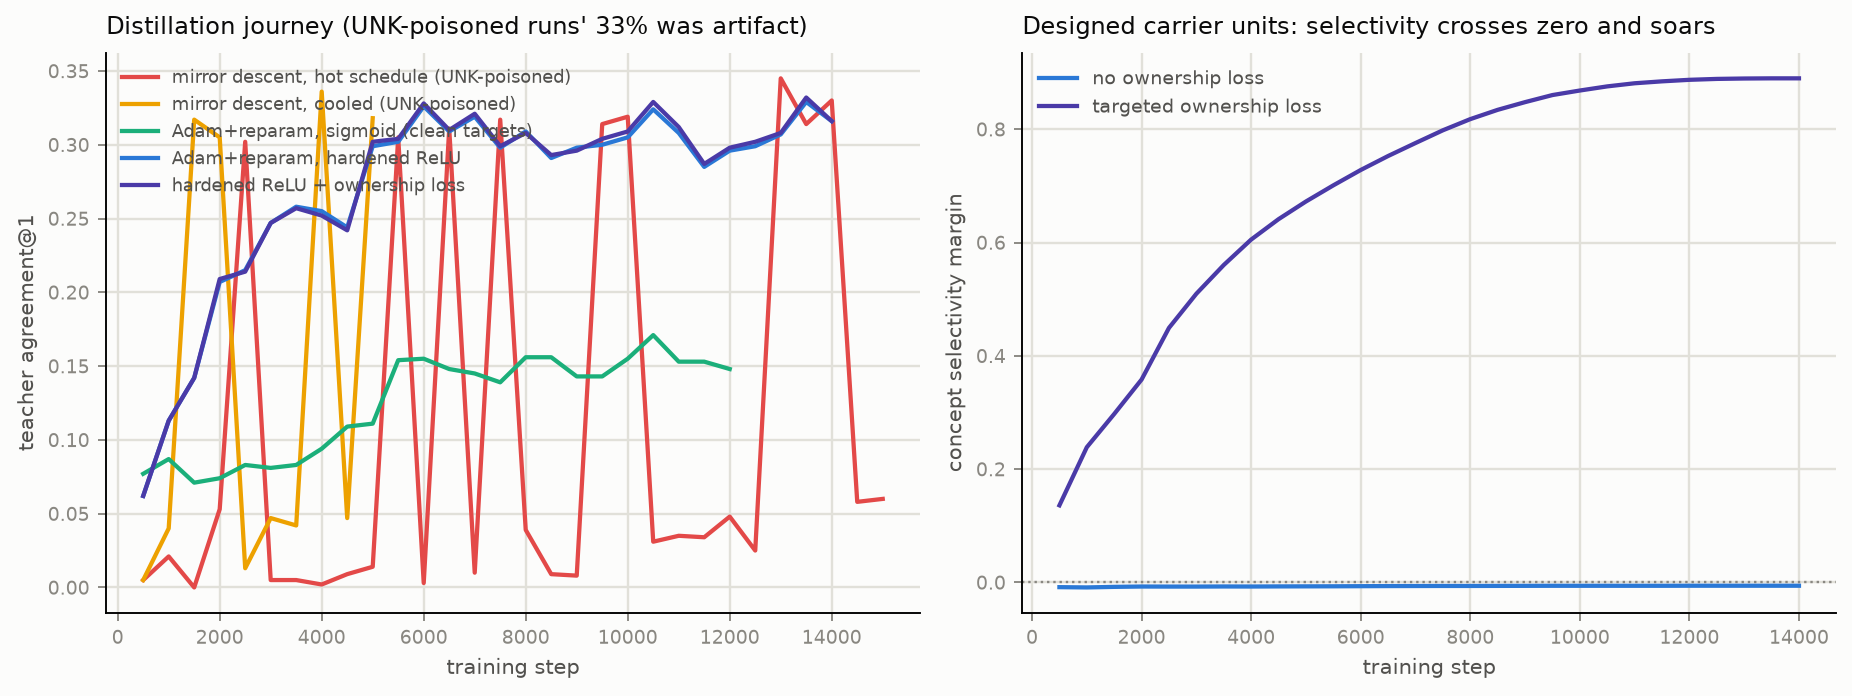
\includegraphics[width=\textwidth]{fig_distill.png}
\caption{Left: the five-run distillation journey (the early ``33\%'' runs
were UNK artifacts). Right: the targeted ownership loss drives concept
selectivity from never-positive to $+0.89$ at zero agreement cost.}
\end{figure}

\section{Lens results}
\textbf{Exactness.} For piecewise-linear activations the exact lens
\emph{reconstructs the forward pass} (max err $3{\times}10^{-7}$): the
lens is not a probe of the computation, it is the computation. For sigmoid
students it remains the exact per-input Jacobian but reads locally ---
\emph{ReLU: exact decomposition, risks dying; sigmoid: lives, local-only.}
The hardened-ReLU recipe resolves the tension.

\textbf{The averaged-lens measurement (headline).} Scoring Anthropic-style
corpus-averaged lenses against computable ground truth:

\begin{center}\small\begin{tabular}{@{}lll@{}}\toprule
Student & input-dependent transport & averaged-lens top-5 overlap\\
\midrule
sigmoid & 1024/1024 (continuous) & \textbf{3.1\%}\\
hardened ReLU & 926/1024 gating & \textbf{91.2\%} (min 20\%)\\
\bottomrule\end{tabular}\end{center}

Fitted-lens fidelity is \textbf{model-regime-dependent} --- from useless
to excellent within one architecture family --- and only a readable
substrate can measure which regime a model is in.

\section{Workspace signatures}
\textbf{Reportable}: pre-output concept dispositions correlate with the
teacher's log-probability of the concept (Spearman $+0.33$ Lily, $+0.27$
park), rising with student quality. \textbf{Controllable}: every
intervention's effect predicted exactly before execution (4 decimals,
every test). \textbf{Causal --- the dragon neuron}: a targeted ownership
loss (maximize each concept's \emph{exclusive-max} margin at its best
unit; the unit-centric variant fails, entrenching frequent tokens) drove
selectivity $-0.008 \to +0.89$ at zero cost. Unit 35 now carries
`` dragon'' at path weight 0.836. Ablate: $p(\mathrm{dragon}) \to 0$.
Boost: $0.0002 \to \mathbf{1.0000}$ (predicted $+0.6615$ = measured).
Generation: babble $\to$ ``dragon dragon dragon...'' Designed, named,
precision-steerable concept neurons, created with a loss term.

\begin{figure}[h]\centering
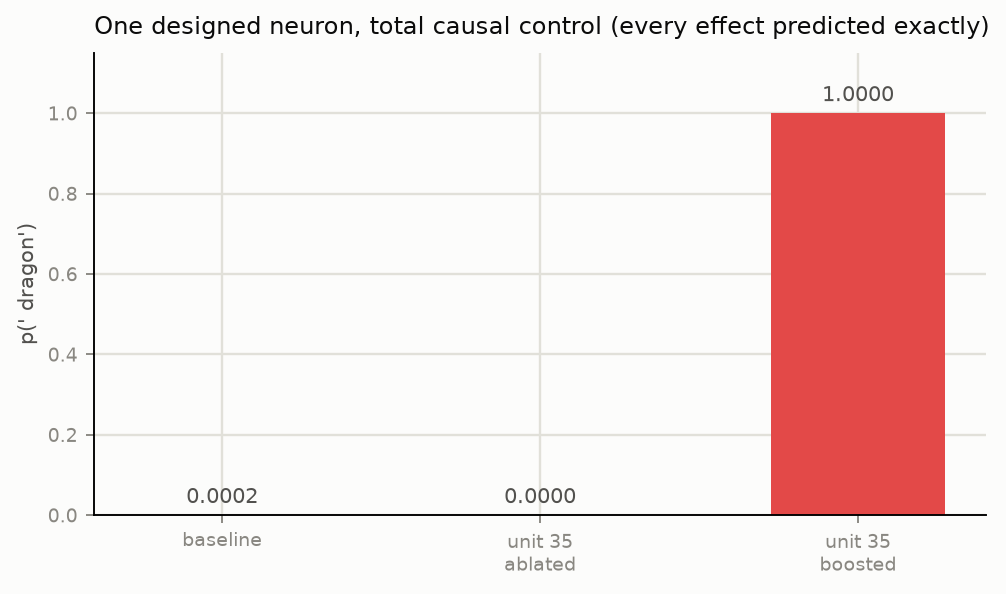
\includegraphics[width=.55\textwidth]{fig_dragon.png}
\caption{Total causal control through one designed neuron.}
\end{figure}

\section{Does ownership decouple? (controlled experiment)}
Single-run observation: dragon's reportable correlation dropped to
$\sim$0 after it gained a dedicated unit. Crossed design: twin models,
identical except which three concepts get ownership; every concept
measured owned and unowned on a shared 2{,}048-prompt set.

Manipulation check: owned concepts reach selectivity $+0.93..+0.99$;
unowned stay $\sim$0.

\begin{center}\small\begin{tabular}{@{}lrrrr@{}}\toprule
concept & $\rho$ owned & $\rho$ unowned & sel owned & sel unowned\\
\midrule
` Lily' & $+0.322$ & $+0.379$ & $+0.979$ & $-0.006$\\
` dragon' & $+0.033$ & $+0.155$ & $+0.983$ & $-0.011$\\
` happy' & $+0.192$ & $+0.172$ & $+0.925$ & $-0.011$\\
` scared' & $+0.191$ & $+0.178$ & $+0.993$ & $+0.007$\\
` park' & $+0.264$ & $+0.231$ & $+0.971$ & $+0.114$\\
` mom' & $+0.076$ & $+0.038$ & $+0.984$ & $+0.024$\\
\bottomrule\end{tabular}\end{center}

\textbf{Paired effect: mean $-0.013$, mixed signs — no systematic
decoupling.} Designed carriers coexist with natural readability. The
dragon drop replicates in sign ($-0.122$, largest single effect) but is
not a law — possibly rare-concept-specific; flagged for a
frequency-stratified follow-up. Practical upshot: ownership engineering is
safe to combine with reportability.

\section{j-carve: certified pruning of self-reflective reasoners}
Task relevance is computable in fixed units (exact-lens path mass toward a
task's answer tokens), so pruning everything outside a task's J-space
yields a small \emph{legal} unit-net that still performs the task, still
reports its dispositions, and carries a \textbf{certified error bound}
(every discarded path's maximum contribution is bounded by the geometry).

\begin{center}\small\begin{tabular}{@{}llll@{}}\toprule
Task & Teacher & Student full & Carved @ 10\% kept\\\midrule
pos-slot (verb/noun) & 1.00 & \textbf{1.00} & \textbf{1.00} ---
$\approx$50$\times$ smaller\\
sentiment & 0.92 & 0.50 (chance) & capacity-gated\\
topic & 1.00 & 0.33 (chance) & capacity-gated\\
pronoun gender & 1.00 & 0.50 (chance) & capacity-gated\\
\bottomrule\end{tabular}\end{center}

The pos-slot reasoner holds 100\% accuracy down to 10\% of the network
(cliff below 5\%). The other tasks are at chance \emph{in the full
student}: a capacity boundary drawn precisely by the teacher reference,
and a roadmap --- each point of student quality unlocks more of the
12-task ladder (\texttt{j-carve/TASKS.md}; Winograd schemas as the
designed negative control: the J-space a task refuses to release is a
compositionality meter).

\begin{figure}[h]\centering
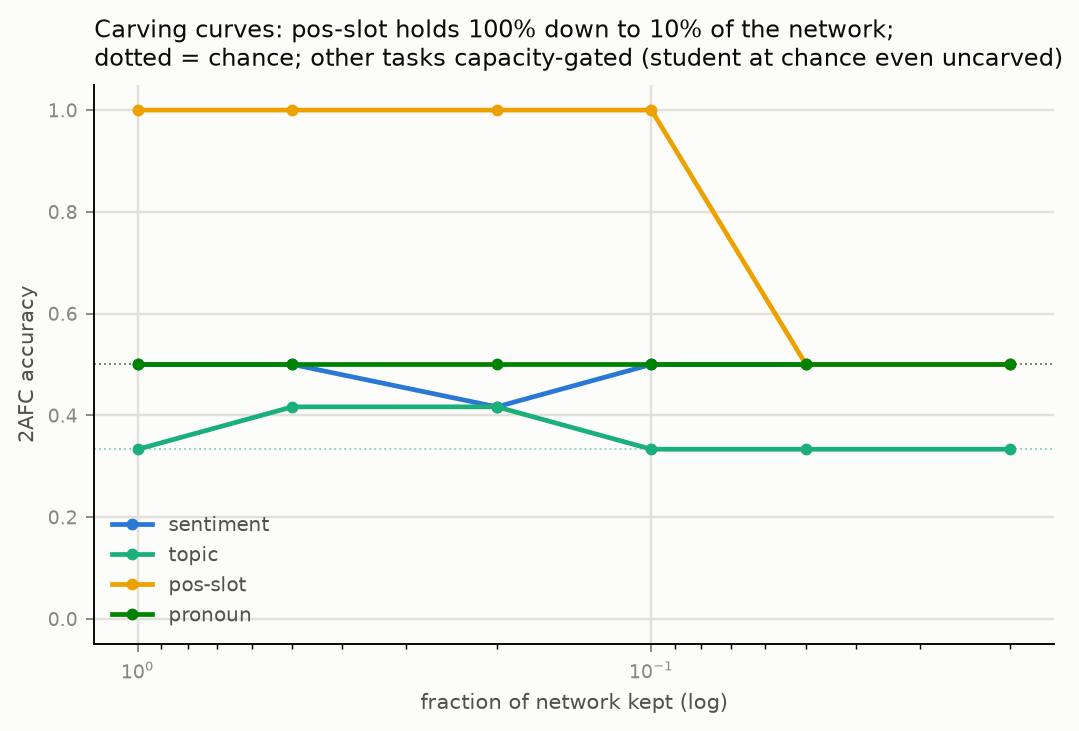
\includegraphics[width=.72\textwidth]{fig_carve.png}
\caption{Carving curves. pos-slot: full accuracy to 10\% kept; dotted
lines are chance; remaining tasks capacity-gated.}
\end{figure}

\section{Standing conclusions}
(1) The unit-net J-space is exact where a transformer's must be
approximated, and approximation fidelity is model-regime-dependent
(3\% vs 91\%) --- measurable only here. (2) Workspace phenomena reproduce
in a readable 3M-parameter substrate with closed-form interventions.
(3) Concept carriers can be designed in by loss engineering, yielding
total, exactly-predicted causal control. (4) Task reasoners carve out of
J-space with certified bounds ($\approx$50$\times$ at zero loss on the
pilot's in-competence task). (5) Every failure had structure: UNK-mass
poisoning, the lazy-linear minimum, mirror-descent oscillation --- each
documented with its fix.

\textbf{Next}: scaled student to unlock carve Tiers 1--2; exact-vs-fitted
against \texttt{anthropics/jacobian-lens} itself; graded clamps for fluent
steering; ownership-decoupling follow-ups (\S6).

\end{document}
